\documentclass[10pt]{article}

\usepackage[margin=1in]{geometry}
\usepackage{graphicx}
\usepackage{booktabs}
\usepackage{amsmath, amssymb}
\usepackage{hyperref}
\usepackage{subcaption}
\usepackage{microtype}
\usepackage{xcolor}
\usepackage{adjustbox}
\usepackage{placeins}

\graphicspath{{../../reports/paper_assets_v0/figures/}}
\newcommand{\tablepath}{tables/}

\title{
Selective Predictive State Models: \\
Reliability and Value-of-Computation under Controlled Interventions
}

\author{
Malo de Pastor \\
Télécom SudParis / ESA Phi-Lab \\
\texttt{malo.depastor@telecom-sudparis.eu}
}

\date{}

\begin{document}
\maketitle

\begin{abstract}
World models are usually evaluated by predictive accuracy alone, but deployment requires knowing when predictions are reliable and when additional computation is useful.
We study this question in a controlled exact-intervention latent-dynamics benchmark.
Each visual simulator state is paired with multiple actions and future observations, encoded with frozen DINOv2 patch tokens, and evaluated through hard-negative latent-displacement ranking.
A spatial action-conditioned Transformer learns state-action dynamics under state-disjoint splits, while action-only and state-only ablations capture only partial structure.
Controlled OOD shifts reveal that constrained environment geometry, rather than horizon or action magnitude alone, drives reliability degradation.
Finally, we study value-of-computation routing between a small full state-action model and a larger full model.
We show that confidence alone is insufficient, while simple context-aware routing better decides when expensive prediction helps or hurts.
\end{abstract}

\section{Introduction}

A useful world model should not only predict future states.
It should also estimate when those predictions are reliable, when the future is identifiable from the available information, and when additional predictive computation is worth paying for.

This work studies that problem in a controlled latent-dynamics setting.
Rather than immediately scaling to open-ended environments, we construct an exact-intervention benchmark where the causal structure is known: for each simulator state, several actions are applied from the same reset state, producing multiple counterfactual futures.
The resulting task is to predict the correct future latent displacement given the current visual state and action.

Our central question is:

\begin{quote}
Can a latent predictive-state model learn action-grounded dynamics, remain reliable under controlled distribution shift, and selectively decide when expensive predictive computation is useful?
\end{quote}

\paragraph{Contributions.}
We make four contributions:
\begin{enumerate}
    \item an exact-intervention latent-dynamics benchmark based on PyBullet and frozen DINOv2 patch-token representations;
    \item a state-disjoint hard-negative ranking protocol that separates action grounding from state-geometry discrimination;
    \item a controlled OOD reliability analysis showing that constrained environment geometry induces a specific failure mode;
    \item a value-of-computation study showing that context-aware routing can outperform naive confidence routing when deciding whether to use a larger predictive model.
\end{enumerate}

\section{Benchmark and Protocol}

\subsection{Exact-intervention environment}

Each simulator state is reset exactly and evaluated under several discrete actions.
This produces multiple future observations from the same initial state.
This intervention structure allows us to distinguish genuine state-action dynamics from correlations induced by observational trajectories.

\subsection{Latent representation}

RGB observations are encoded with a frozen DINOv2 ViT-S/14 encoder.
We use patch-token representations and pool them from a $16 \times 16$ grid to a $4 \times 4$ grid.
The model predicts latent displacements:
\[
\Delta z = z_{t+1} - z_t.
\]

\subsection{Hard-negative ranking}

Given a current latent state $z_t$ and action $a_t$, the model predicts a future displacement $\hat{\Delta z}$.
The evaluation ranks the correct future displacement against hard negatives.

We use two key negative types:
\begin{itemize}
    \item same-state/different-action negatives, testing action discrimination;
    \item same-action/different-state negatives, testing state-geometry discrimination.
\end{itemize}

We report strict top-1, tie-aware top-1, and pairwise margin decompositions.
Stay actions are excluded from the main moving-only evaluation because their true latent displacement can be non-identifiable.

\section{Action-Grounded Latent Dynamics}

The full spatial action-conditioned Transformer reaches near-perfect performance under the state-disjoint exact-intervention protocol.
Ablations show that action-only and state-only models each capture only partial structure, while the full model combines both axes.

\paragraph{Claim.}
Under exact interventions and state-disjoint evaluation, the model learns genuine state-action latent dynamics rather than exploiting a single shortcut.

\section{Controlled OOD Reliability}

We evaluate the frozen v5.2 full model under controlled OOD variants.
The results show that horizon-only and velocity-only shifts preserve high performance, while increasing the number of blocked directions creates a substantial drop.

\begin{figure}[t]
    \centering
    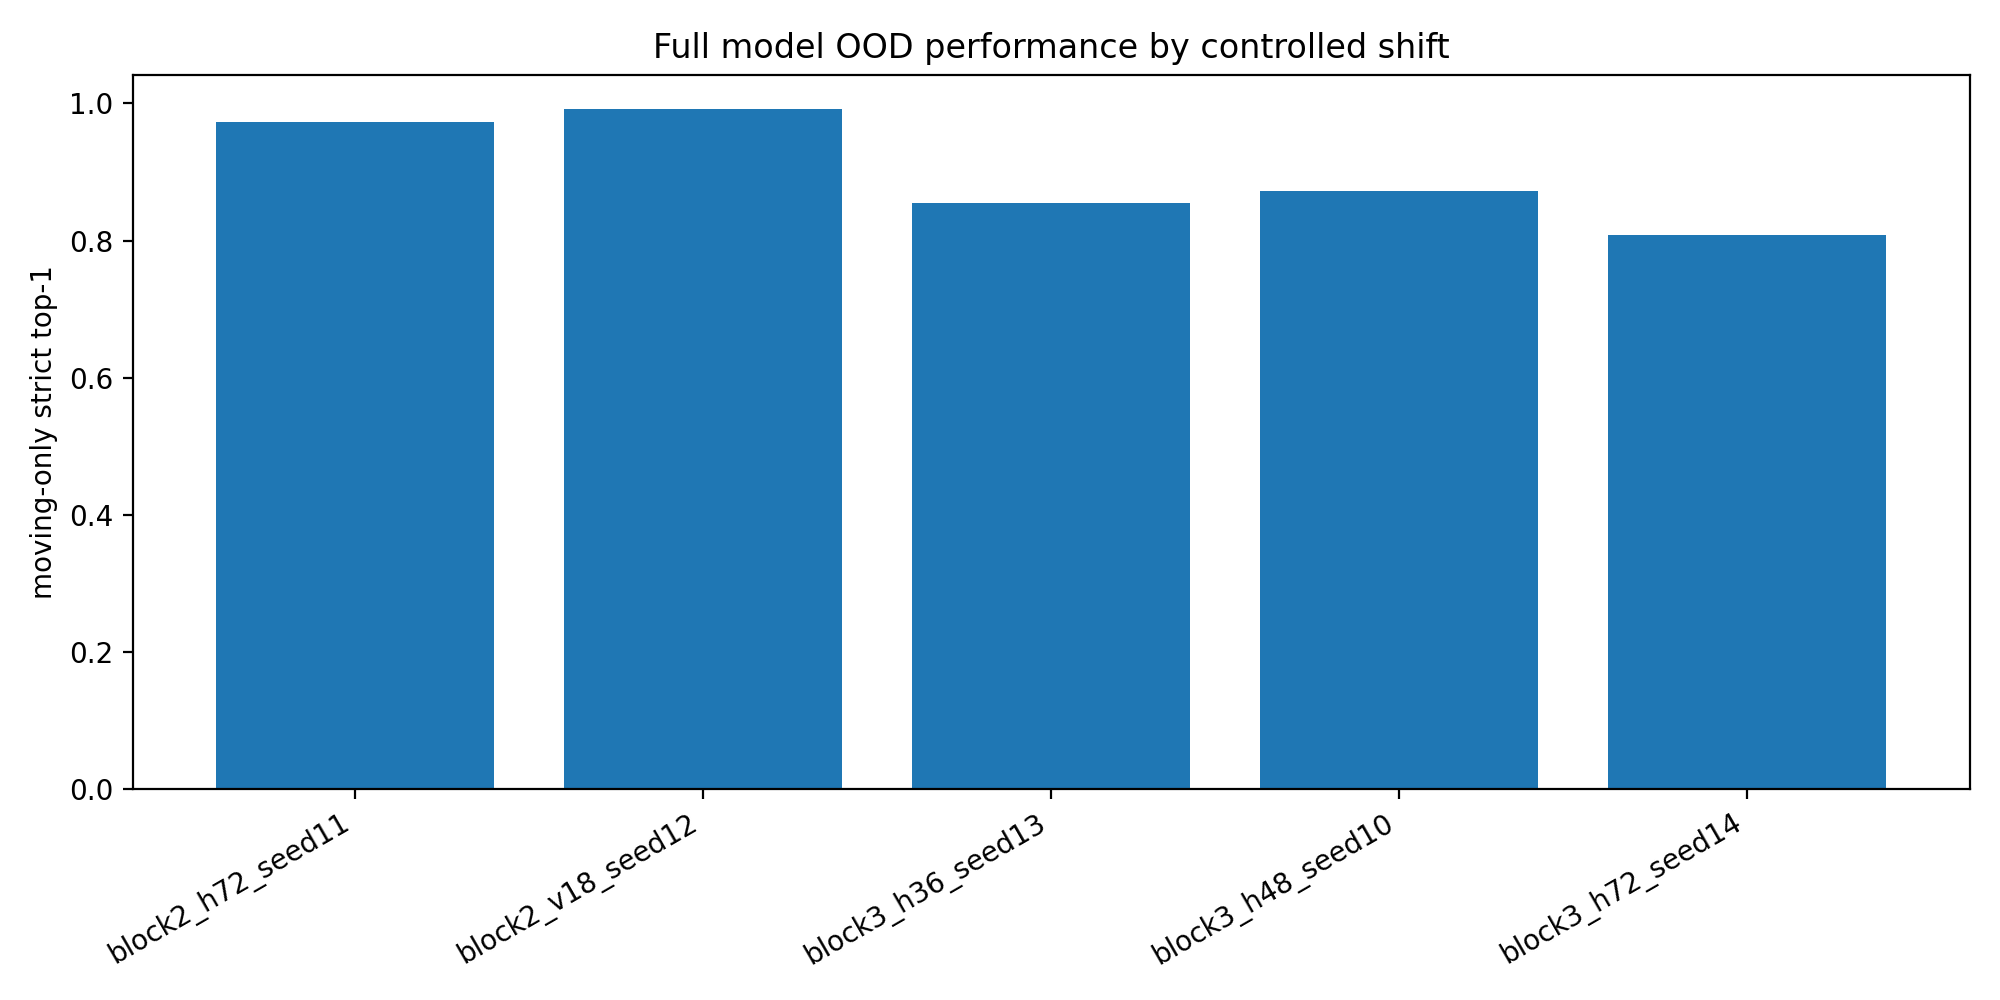
\includegraphics[width=0.85\linewidth]{fig_v5_3_ood_top1_by_variant.png}
    \caption{
    Controlled OOD performance of the full model.
    Horizon-only and velocity-only shifts are mild, while block3 variants expose a stronger failure mode.
    }
    \label{fig:ood_top1}
\end{figure}

\begin{table}[t]
\centering
\small
\resizebox{\linewidth}{!}{%
\begin{tabular}{lrrrrr}
\toprule
Variant & Top-1 & Same-action & Same-state & @80\% cov. & @60\% cov. \\
\midrule
block2\_h72\_seed11 & 0.972756 & 0.987580 & 0.985978 & 0.995000 & 1.000000 \\
block2\_v18\_seed12 & 0.992386 & 0.996616 & 0.998731 & 0.977500 & 1.000000 \\
block3\_h36\_seed13 & 0.854931 & 0.884271 & 0.982885 & 0.865000 & 0.966667 \\
block3\_h48\_seed10 & 0.872305 & 0.903399 & 0.992952 & 0.874167 & 0.975555 \\
block3\_h72\_seed14 & 0.807910 & 0.847054 & 0.983051 & 0.821667 & 0.937778 \\
\bottomrule
\end{tabular}%
}
\caption{Controlled OOD evaluation of the full state-action Transformer. The strongest degradation occurs under block3 shifts, especially on the same-action/different-state axis.}
\label{tab:ood_summary}
\end{table}


\paragraph{Interpretation.}
The model is not generically fragile.
It remains action-grounded under several shifts, but constrained geometry degrades same-action/different-state discrimination.
This suggests that reliability depends on state-geometry complexity.

\section{A Meaningful Value-of-Computation Setup}

Early experiments with action-only, state-only, and no-context cheap models reveal a large oracle gap, but these models are too incomplete to serve as realistic cheap predictors.
We therefore train a smaller full state-action Transformer with model dimension 128, one layer, and four heads.

\begin{figure}[t]
    \centering
    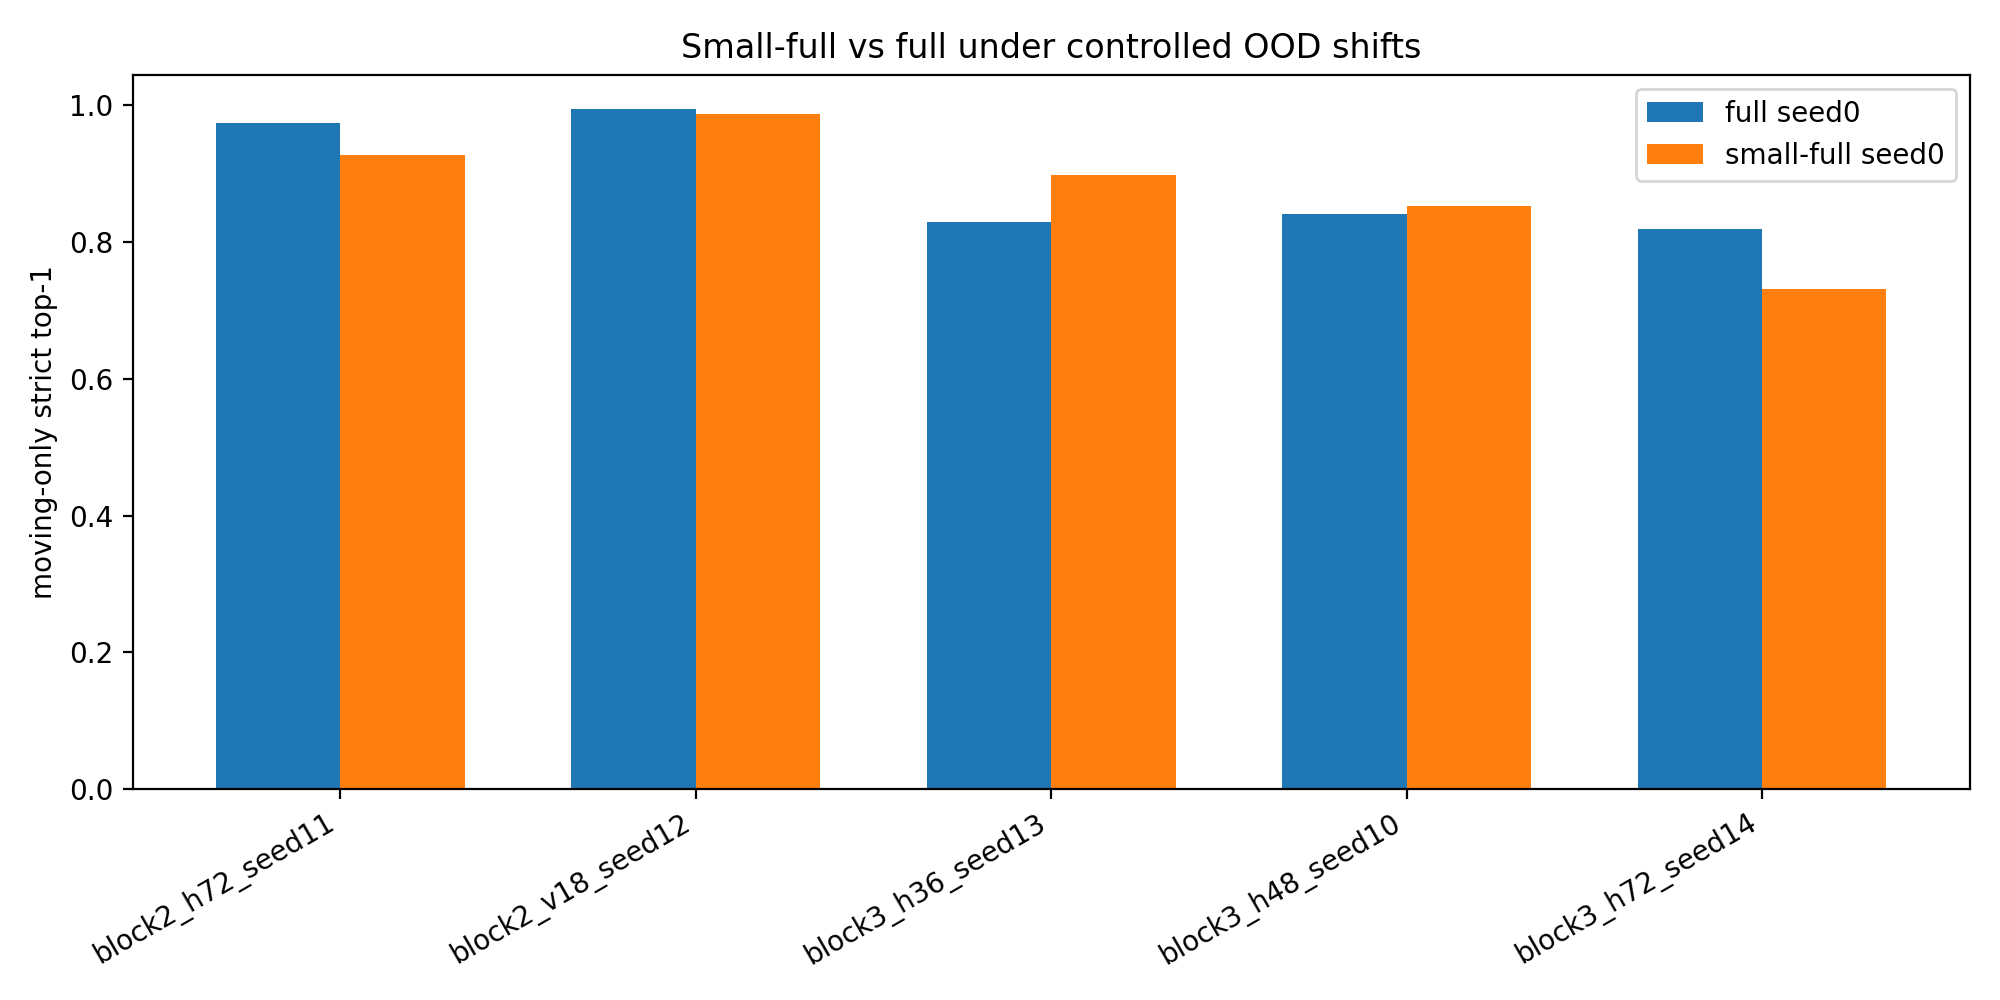
\includegraphics[width=0.85\linewidth]{small_full_vs_full_ood.png}
    \caption{
    Small full model versus larger full model under OOD shifts.
    The expensive model is not uniformly better, making value-of-computation non-trivial.
    }
    \label{fig:small_vs_full}
\end{figure}

\begin{table}[t]
\centering
\small
\resizebox{\linewidth}{!}{%
\begin{tabular}{lrrrr}
\toprule
Variant & Full mean & Full seed0 & Small-full & Gap \\
\midrule
block2\_h72\_seed11 & 0.972756 & 0.974 & 0.928 & 0.046 \\
block2\_v18\_seed12 & 0.992386 & 0.995 & 0.987 & 0.008 \\
block3\_h36\_seed13 & 0.854931 & 0.829 & 0.897 & -0.068 \\
block3\_h48\_seed10 & 0.872305 & 0.841 & 0.853 & -0.012 \\
block3\_h72\_seed14 & 0.807910 & 0.818 & 0.731 & 0.087 \\
\bottomrule
\end{tabular}%
}
\caption{Comparison between the reduced full model and the larger full model. The expensive model is not uniformly better, making value-of-computation non-trivial.}
\label{tab:small_full}
\end{table}


The small full model remains strong on ID and easy OOD settings, and is sometimes better than the larger model.
However, the larger model helps in harder regimes such as block3 with longer horizon.
Thus the compute decision is not trivial:
\[
\text{route to expensive model} \quad \Longleftrightarrow \quad
\text{gain}_{\text{full} - \text{small}} > \lambda.
\]

\section{Context-Aware Value-of-Computation Routing}

We compare cheap-only, full-only, oracle routing, confidence-threshold routing, and a context-aware learned gain router.
The router uses cheap-model uncertainty and simple environment context features such as horizon and velocity.

\begin{figure}[t]
    \centering
    \begin{subfigure}{0.48\linewidth}
        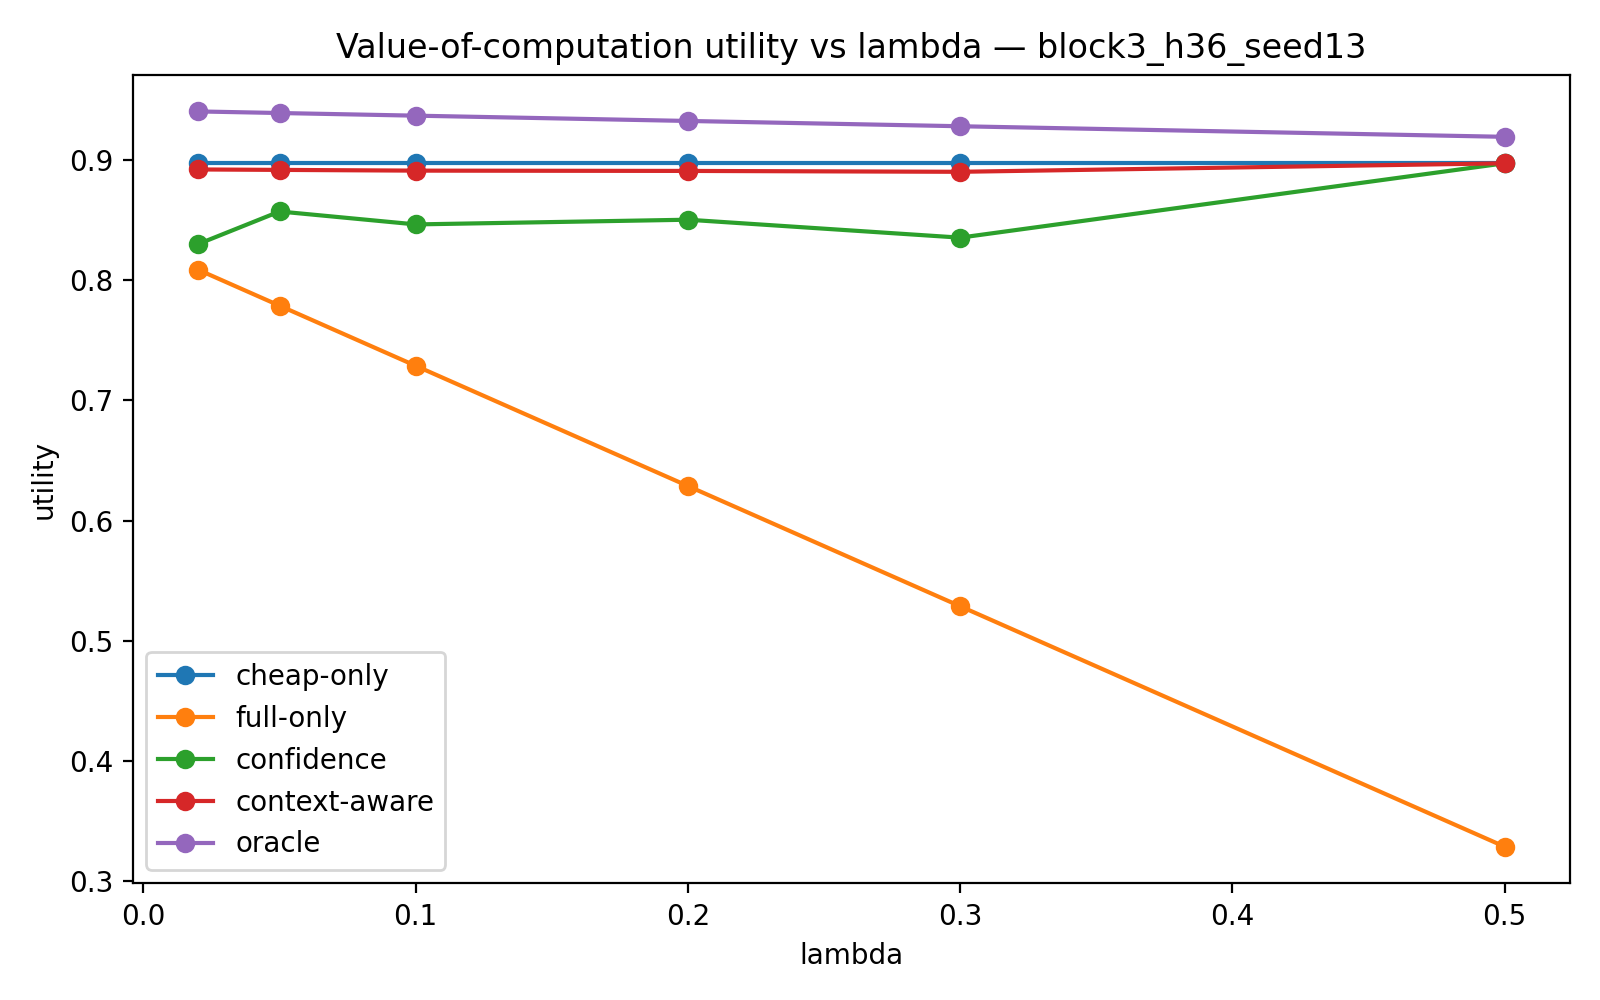
\includegraphics[width=\linewidth]{fig_v5_8_utility_vs_lambda_block3_h36_seed13.png}
        \caption{block3\_h36}
    \end{subfigure}
    \begin{subfigure}{0.48\linewidth}
        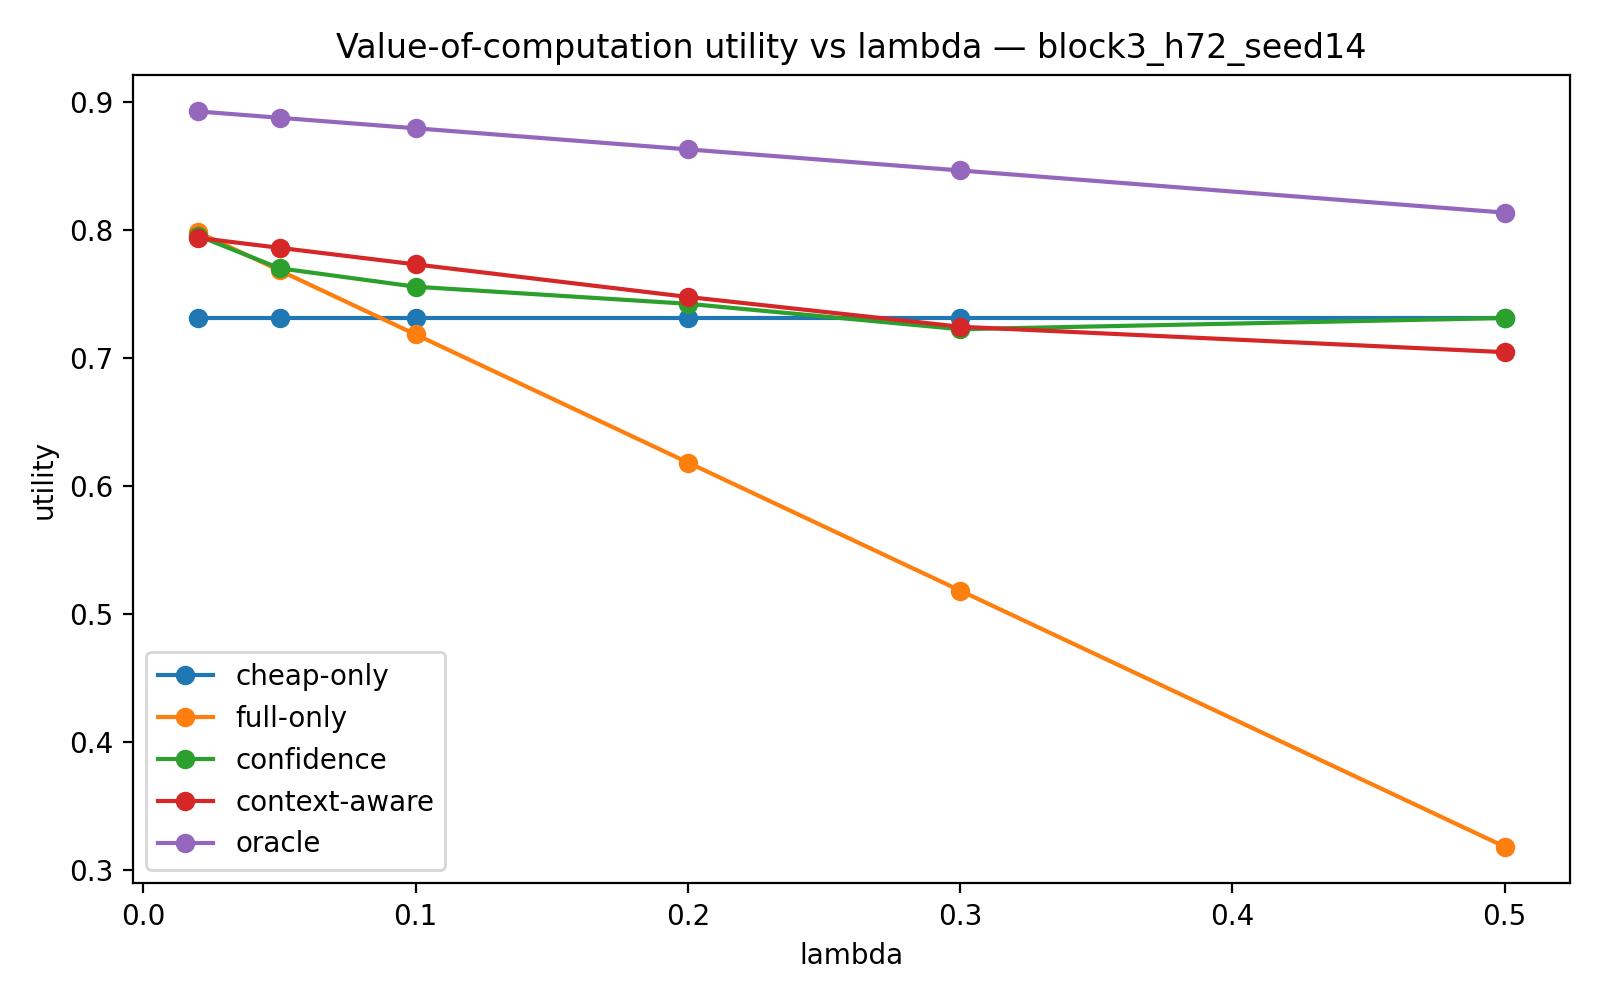
\includegraphics[width=\linewidth]{fig_v5_8_utility_vs_lambda_block3_h72_seed14.png}
        \caption{block3\_h72}
    \end{subfigure}
    \caption{
    Utility versus compute cost $\lambda$.
    On block3\_h36, the small model is safer and the router avoids the expensive model.
    On block3\_h72, the expensive model helps more often and the router improves over confidence routing.
    }
    \label{fig:voc_utility}
\end{figure}

\begin{figure}[t]
    \centering
    \begin{subfigure}{0.48\linewidth}
        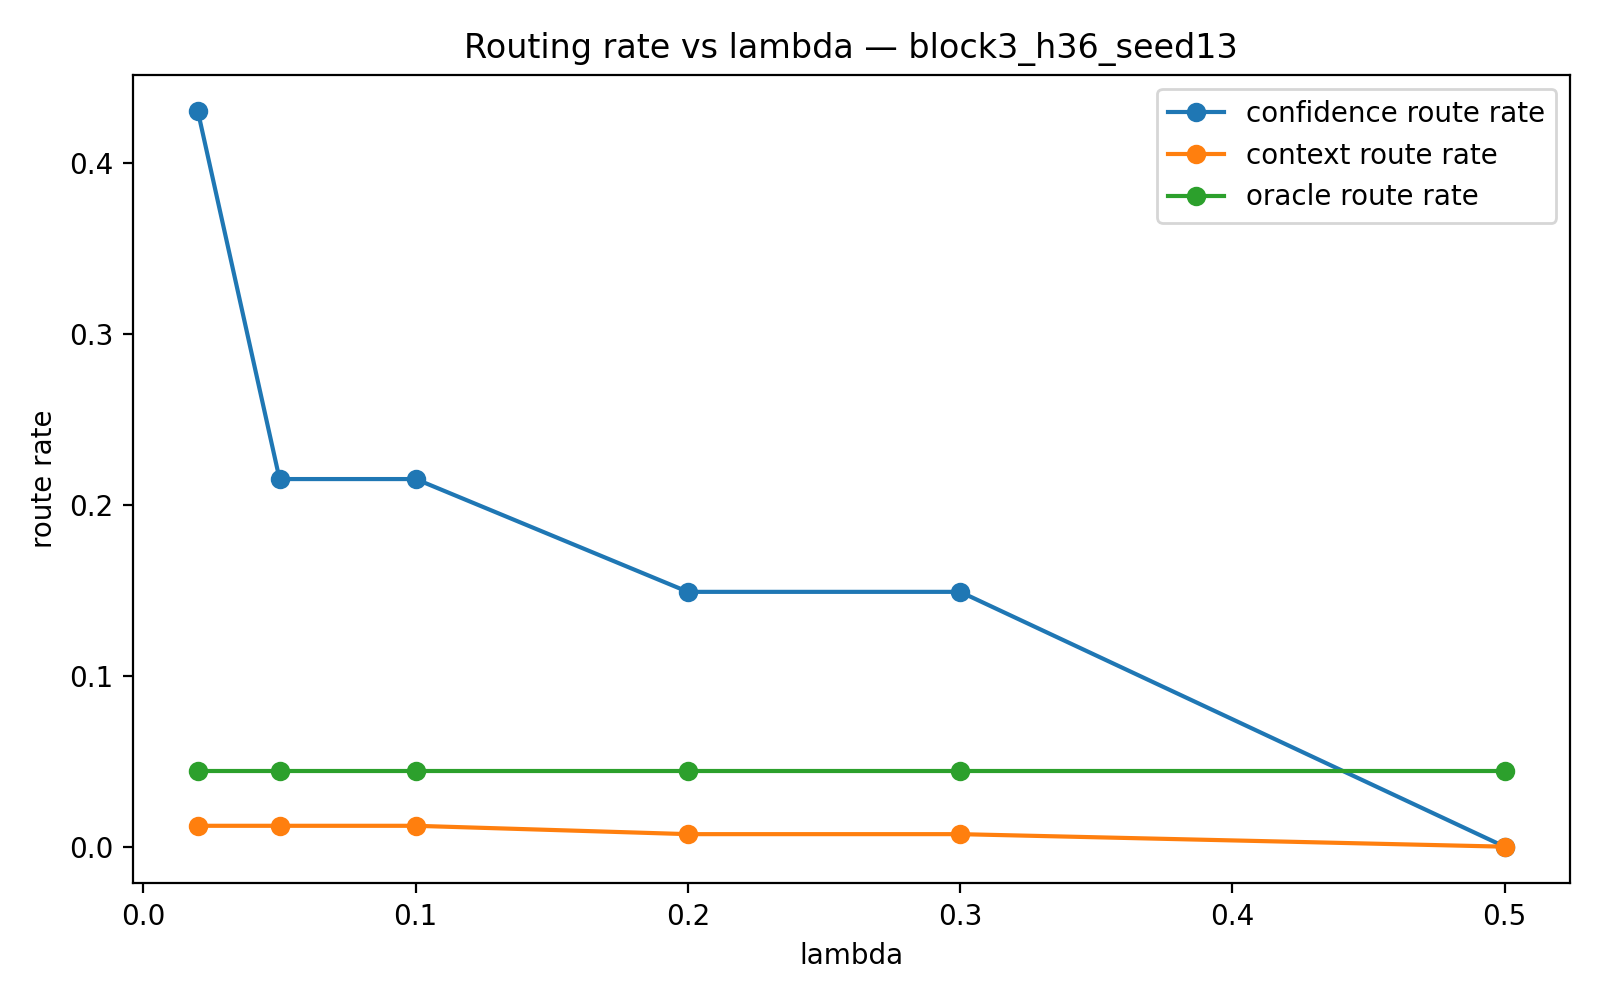
\includegraphics[width=\linewidth]{fig_v5_8_route_rate_vs_lambda_block3_h36_seed13.png}
        \caption{block3\_h36}
    \end{subfigure}
    \begin{subfigure}{0.48\linewidth}
        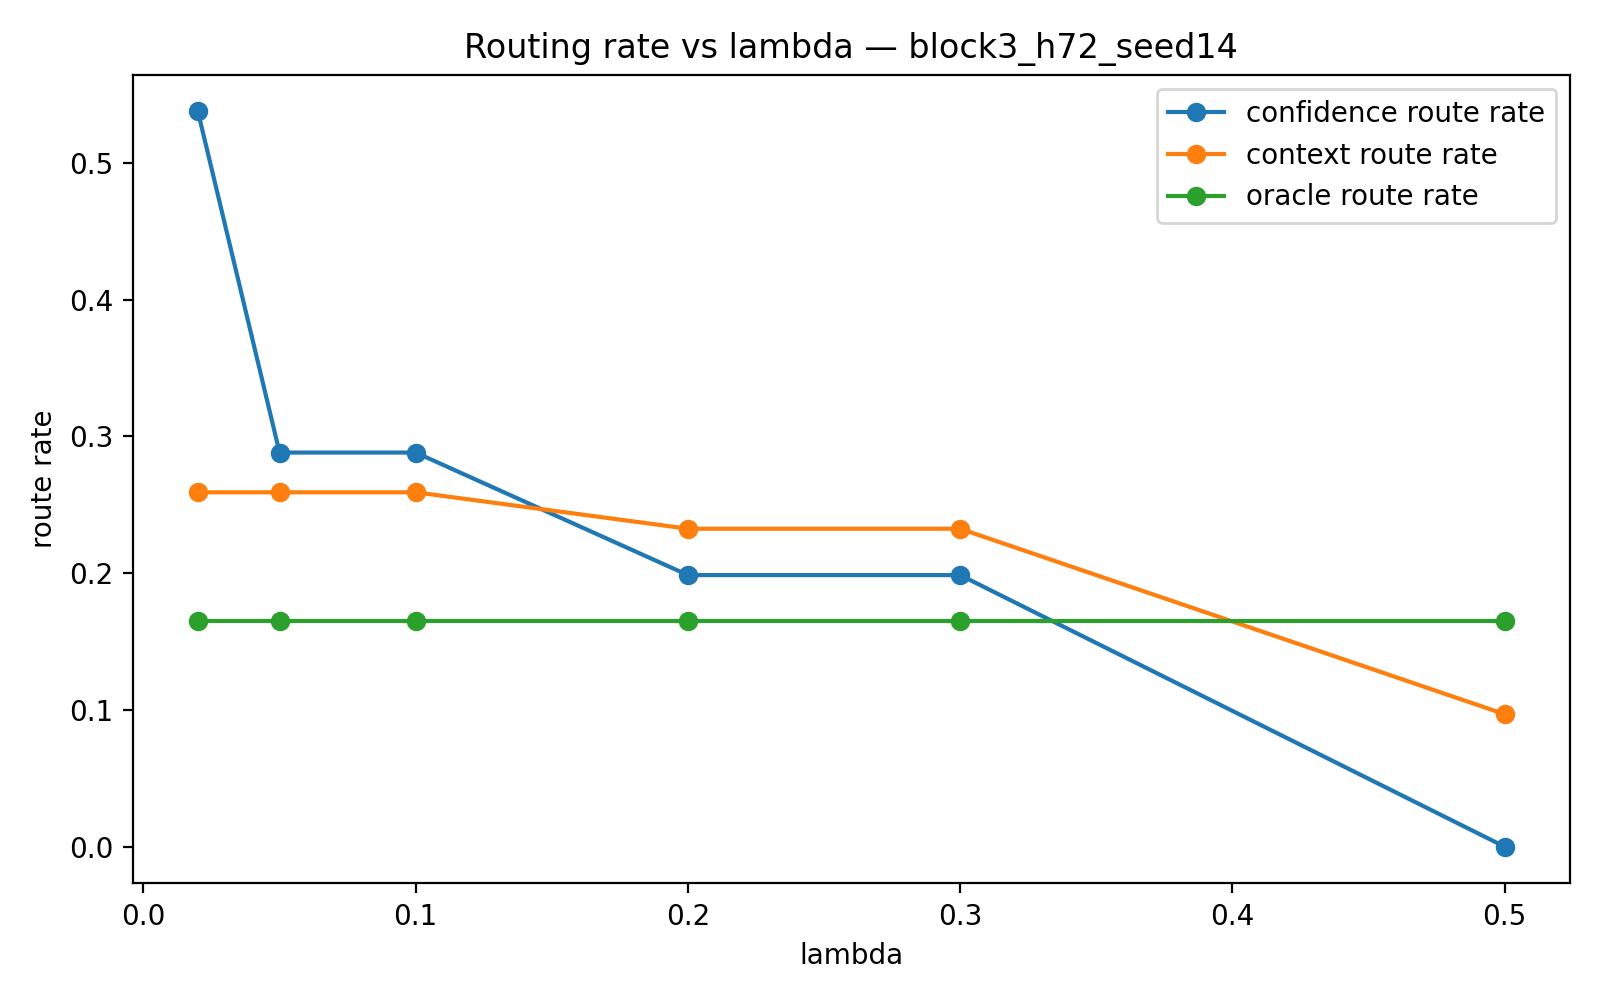
\includegraphics[width=\linewidth]{fig_v5_8_route_rate_vs_lambda_block3_h72_seed14.png}
        \caption{block3\_h72}
    \end{subfigure}
    \caption{
    Routing rates versus compute cost.
    The context-aware router routes differently depending on the environment regime.
    }
    \label{fig:voc_route_rate}
\end{figure}

\paragraph{Key result.}
Value-of-computation is not captured by confidence alone.
It depends on the interaction between model uncertainty and environment context.
Table~\ref{tab:routing_key_cases} summarizes the two key regimes: block3\_h36, where the small model should usually be trusted, and block3\_h72, where calling the larger model is often useful.

\begin{table}[t]
\centering
\small
\resizebox{\linewidth}{!}{%
\begin{tabular}{lrrrrrr}
\toprule
Variant & $\lambda$ & Cheap & Full & Conf. & Context & Oracle \\
\midrule
block3\_h36 & 0.10 & 0.897 & 0.729 & 0.846 & 0.891 & 0.937 \\
block3\_h72 & 0.10 & 0.731 & 0.718 & 0.756 & 0.773 & 0.879 \\
block3\_h36 & 0.30 & 0.897 & 0.529 & 0.835 & 0.890 & 0.928 \\
block3\_h72 & 0.30 & 0.731 & 0.518 & 0.723 & 0.724 & 0.846 \\
\bottomrule
\end{tabular}%
}
\caption{Key value-of-computation cases. On block3\_h36, the small model is safer and context-aware routing avoids most harmful calls to the expensive model. On block3\_h72, the expensive model helps more often and context-aware routing improves over cheap-only, full-only, and confidence routing at $\lambda=0.10$.}
\label{tab:routing_key_cases}
\end{table}


\FloatBarrier

\section{Limitations}

This benchmark is synthetic and controlled.
The current router uses only simple context features and remains far from oracle performance.
The OOD space is still limited, and the expensive model is not uniformly more robust.
Future work should include explicit geometry-complexity features, leave-one-shift-out validation, continuous actions, and planning-level evaluation.

\section{Conclusion}

We introduced a controlled exact-intervention setting for studying selective predictive-state models.
The results show that action-grounded latent dynamics can be learned under state-disjoint evaluation, that constrained geometry induces specific OOD reliability failures, and that value-of-computation routing becomes meaningful when both cheap and expensive predictors are competent but not uniformly ordered.
This supports the view that future world models should not only predict: they should also estimate when prediction is reliable and when additional computation is worth paying for.

\FloatBarrier

\bibliographystyle{plain}
\begin{thebibliography}{9}

\bibitem{lecun2022path}
Yann LeCun.
\newblock A Path Towards Autonomous Machine Intelligence.
\newblock 2022.

\bibitem{dinov2}
Maxime Oquab et al.
\newblock DINOv2: Learning Robust Visual Features without Supervision.
\newblock 2023.

\bibitem{selectiveprediction}
Yonatan Geifman and Ran El-Yaniv.
\newblock Selective Classification for Deep Neural Networks.
\newblock NeurIPS, 2017.

\end{thebibliography}

\end{document}
